\documentclass{beamer}

% Theme
%\usetheme{Madrid}
%\usecolortheme{default}
\mode<presentation>
{
  \usetheme{Warsaw}
  \setbeamercovered{transparent}
}

\usetheme{Warsaw}

\setbeamersize{text margin left=3mm}
\setbeamersize{text margin right=3mm}

% Packages
\usepackage[utf8]{inputenc}
\usepackage[backend=bibtex, style=authoryear]{biblatex} % You can change the style if you prefer a different citation style
\addbibresource{Chp1.bib}

\usepackage{dirtytalk}
\usepackage{cancel}
\usepackage{graphicx}
\usepackage{wrapfig}
\usepackage{caption}
\usepackage{booktabs}
\usepackage{adjustbox}
\usepackage{amssymb}


% Title slide
\title[]{Heterogeneous Returns and the Distribution of Wealth}
\author[Edwards]{Decory Edwards}
\institute[JHU]{Johns Hopkins University}
\date{\today}

\begin{document}

\begin{frame}
  \titlepage
\end{frame}

\section{Introduction}

\begin{frame}{A two-way street between macro and inequality \parencite{Ahn2017} :}


Empirically, fiscal policy (i.e. stimulus checks) and aggregate shocks can have differential effects across households.

\begin{itemize}
\item Macro matters for inequality
\end{itemize}
\vspace{2.5mm}

Representative agent models have a difficult time matching empirical estimates of macro variables (MPC and the wealth distribution).

\begin{itemize}
\item Inequality matters for macro
\end{itemize}

Incorporating \textit{heterogeneity across households} can help focus on this second issue.

\end{frame}

\subsection{Literature Review}


\begin{frame}{Key insights from het. agent macro}

    \begin{itemize}
    \item Uninsurable, idiosyncratic risk to income and movements in aggregate productivity \parencite{ks1998}
    % \item Ex-ante heterogeneity in the time preference of households \parencite{cstw2017}
    \item Classifying models with ex-ante and ex-post heterogeneity \parencite{gkgv22}
    \end{itemize}
    
    Income uncertainty helps. So does time preference heterogeneity.

    \vspace{10mm}
    \textbf{Q:} \textit{What other parameters relevant to consumption-saving decisions may be plausibly different across households ex-ante? Do they help better match the wealth distribution?}

\end{frame}
%%%%%%%%%%%%%%%%%%

\begin{frame}{Incorporating estimates of heterogeneous returns}

   \small
   \begin{enumerate}
    \item Comprehensive, administrative tax data in Norway from 2004 to 2015  \parencite{aflgdmlp20}
    \item Documents heterogeneous returns in PSID and structural estimation of a model with skill endowments \parencite{Daminato2024}
    \end{enumerate}
    
    Like time preference het., I find that return het. does well with matching wealth distribution.

\end{frame}
%%%%%%%%%%%%%%%%%%%%%%%%

\begin{frame}{Outline}
\begin{enumerate}
\item Empirical evidence of heterogeneous returns
\item Model of saving with heterogeneous returns
\item Structural estimation of model to match wealth data
\end{enumerate}
\end{frame}
%%%%%%%%%%%%%%%%%%

\subsection{Heterogeneous Returns in the Data}
\begin{frame}{A closer look at \cite{aflgdmlp20}}

   \begin{columns}
     \column{0.5\textwidth}
     \small
     Following optimal portfolio choice theory from Merton (1969) and Samuelson (1969)
    \centering

    \begin{itemize}
    \item Optimal share in the risky asset is given by
    $$ \alpha_{it}^{m} = \frac{\mathbb{E}(r_{t}^{m} - r_{t}^{s})}{\gamma_i \sigma^{2}_{t}}.$$
    \item Individual \textit{realized} return to financial assets can be written as
    $$ r_{it}^{f} = r_{t}^{s} + \alpha_{it}^{m} (r_{t}^{m} - r_{t}^{s}). $$
    \end{itemize}

    \column{0.5\textwidth}
    \centering
    \begin{figure}
    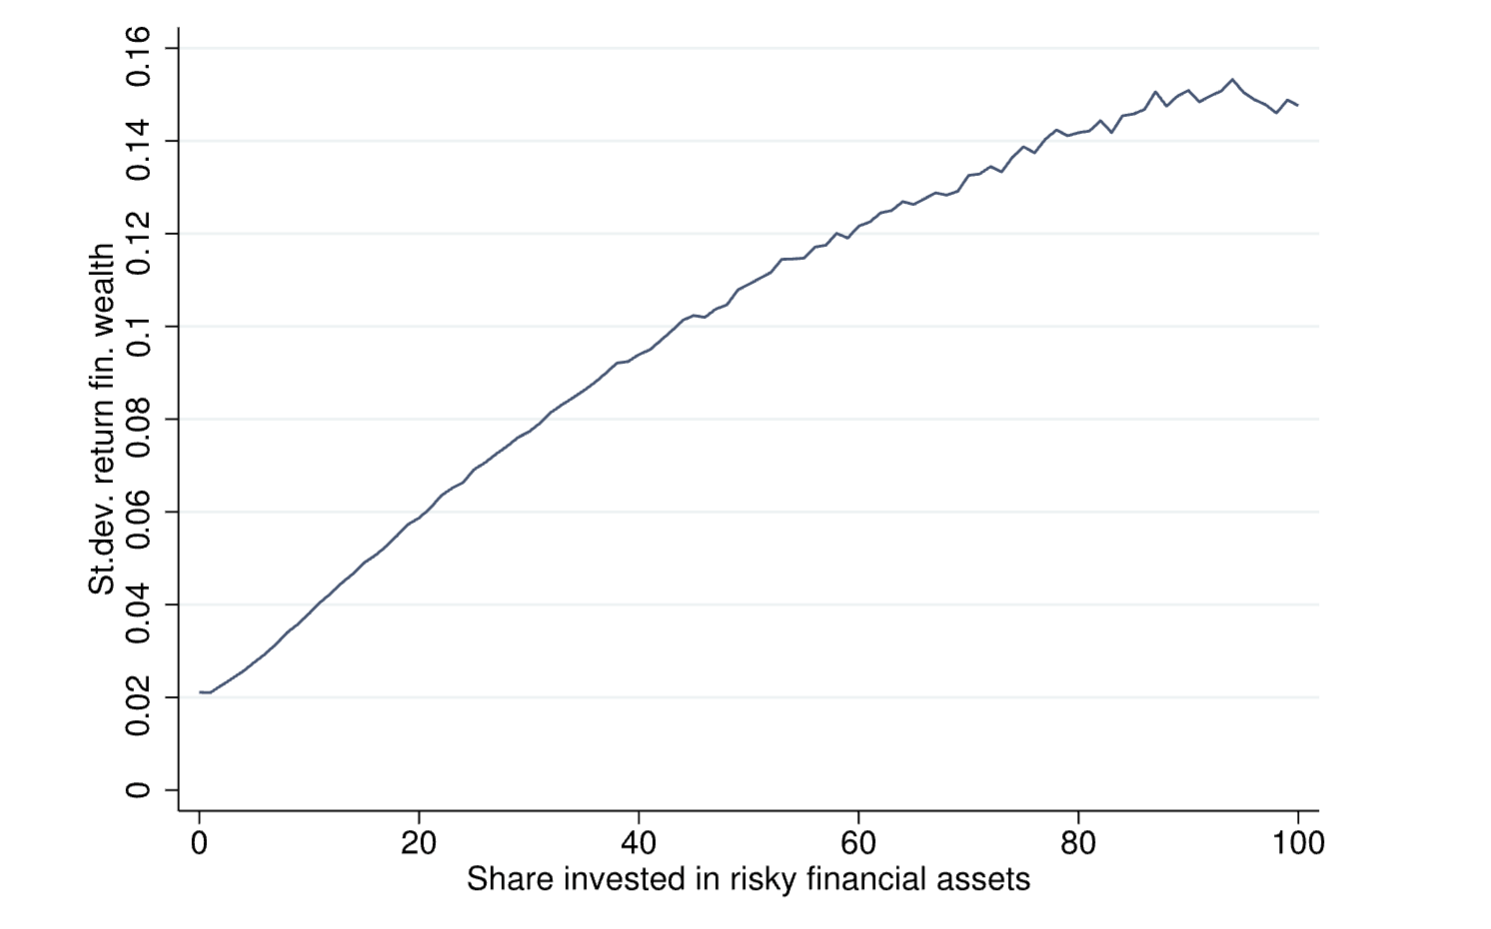
\includegraphics[width=\textwidth]{Figures/Fagereng2020Fig1.png}
    \captionsetup{font=scriptsize}
    \caption{Heterogeneity in returns to financial wealth by share of risky assets from \cite{aflgdmlp20}.}
    \end{figure}
  \end{columns}

\end{frame}
%%%%%%%%%%%%%%%%

\begin{frame}{Empirical estimate of heterogeneity}

     \begin{columns}
     \small
     \column{0.5\textwidth}
    \centering

    \begin{itemize}
    \item Step 1: linear regression for the return to net worth using panel
    $$ r^{n}_{it} = X^{'}_{it} \beta + u_{it}. $$
    \item Step 2: Add fixed effects
    $$ u_{it} = f_{i} + e_{it}. $$
    $\implies R^2$ goes from $.33$ to $.5$.
    \end{itemize}


    \column{0.5\textwidth}
    \centering
    \begin{figure}
    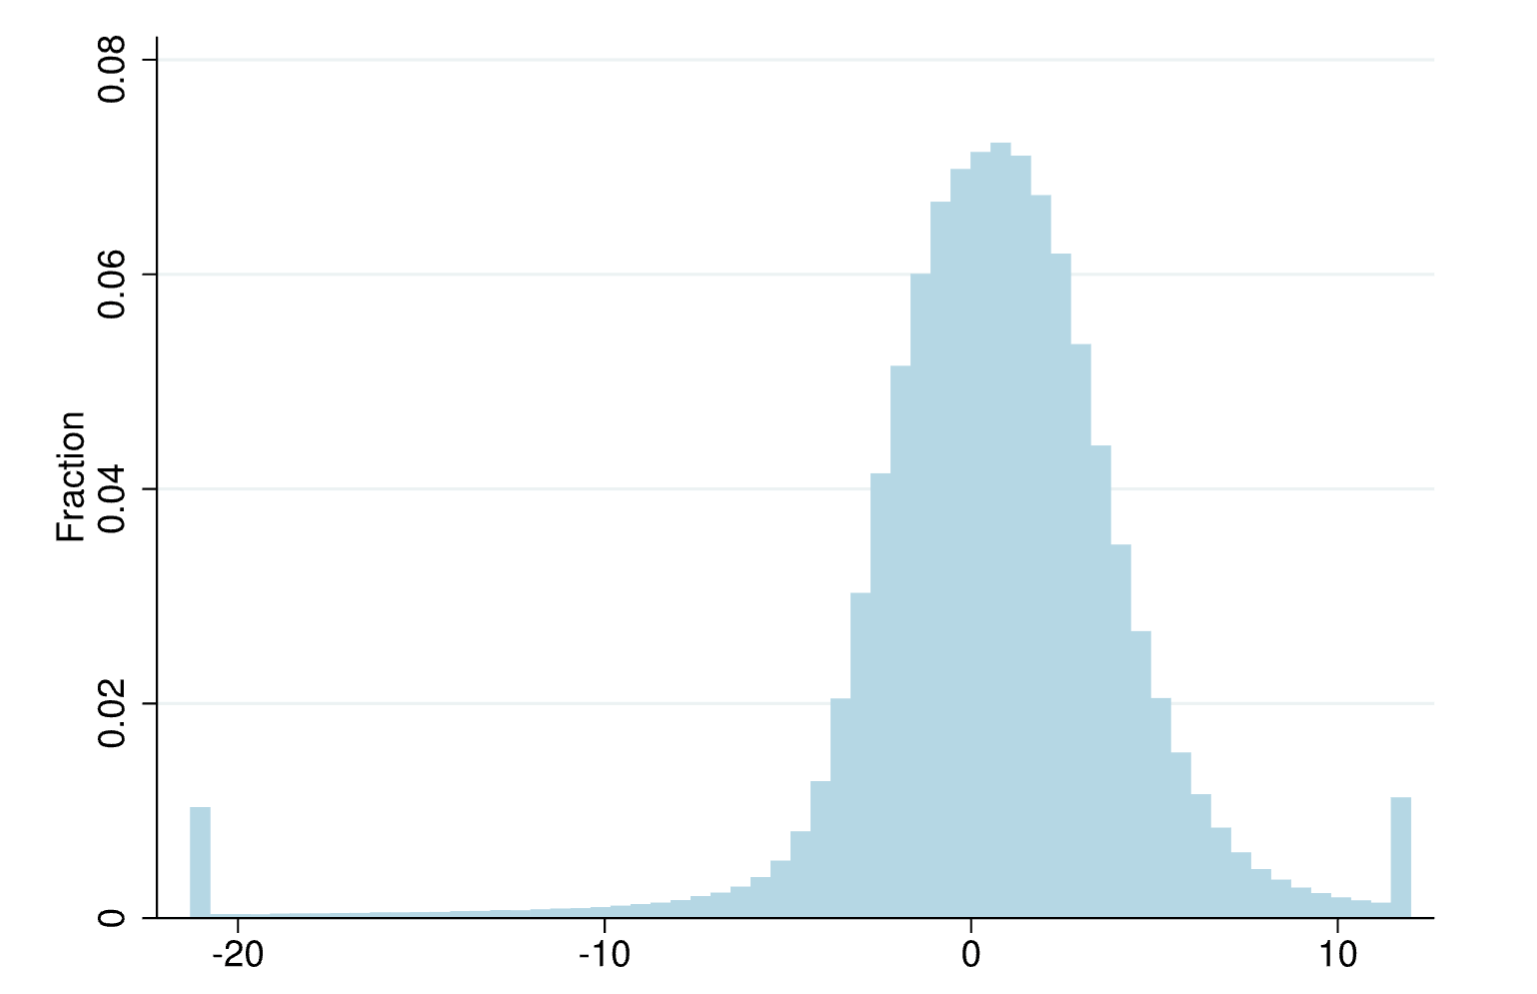
\includegraphics[width=\textwidth]{Figures/Fagereng2020Fig8.png}
    \captionsetup{font=scriptsize}
    \caption{Distribution of fixed effects in the return to net worth from \cite{aflgdmlp20}.}
    \end{figure}
  \end{columns}

\end{frame}
%%%%%%%%%%%%%%%%

\section{Model}
%\subsection{Environment}

\small
\begin{frame}{Labor income process}

\begin{itemize}
\item Household income: $$y_t = p_t \xi_t W_t$$
\item Permanent component: $$p_t = p_{t-1} \psi_t$$
\item Transitory component: $$\xi_t =
    \begin{cases}
       \mu & \text{with probability $\mho$} \\
      (1-\tau_t) \ell \theta_t & \text{with probability $1-\mho$}
   \end{cases}$$
\end{itemize}
%\vspace{1.5mm}

\end{frame}
%%%%%%%%%%%%%%%%%
%Put equations for permanent and transitory income%

\footnotesize
\begin{frame}{(Normalized) Optimization problem}

Choose profiles $\{c_{t_n}\}_{n=0}^{\infty}$ that satisfy
 \begin{eqnarray*}
  v(m_t) &=& \max_{c_t} u(c_t(m_t)) + \beta \cancel{D} \mathbb{E}_{t}[\psi_{t+1}^{1-\rho}v(m_{t+1})] \\
  &\text{s.t.}& \\
  a_t &=& m_t - c_t(m_t), \\
  k_{t+1} &=& \frac{a_t}{\cancel{D}\psi_{t+1}}, \\
  m_{t+1} &=& (\daleth + r_t)k_{t+1} + \xi_{t+1}, \\
  a_t &\geq& 0.
\end{eqnarray*}

Production function $$Y = Z K^{\alpha} (\ell L)^{1-\alpha}$$

\end{frame}
%%%%%%%%%%%%%%%%%

\subsection{Simulation}
%%%%%%%%%%%%%%%%%

\begin{frame}{Calibration}

Standard calibration scheme used to simulate the model.

  \vfill
   \begin{figure}
    \centering
    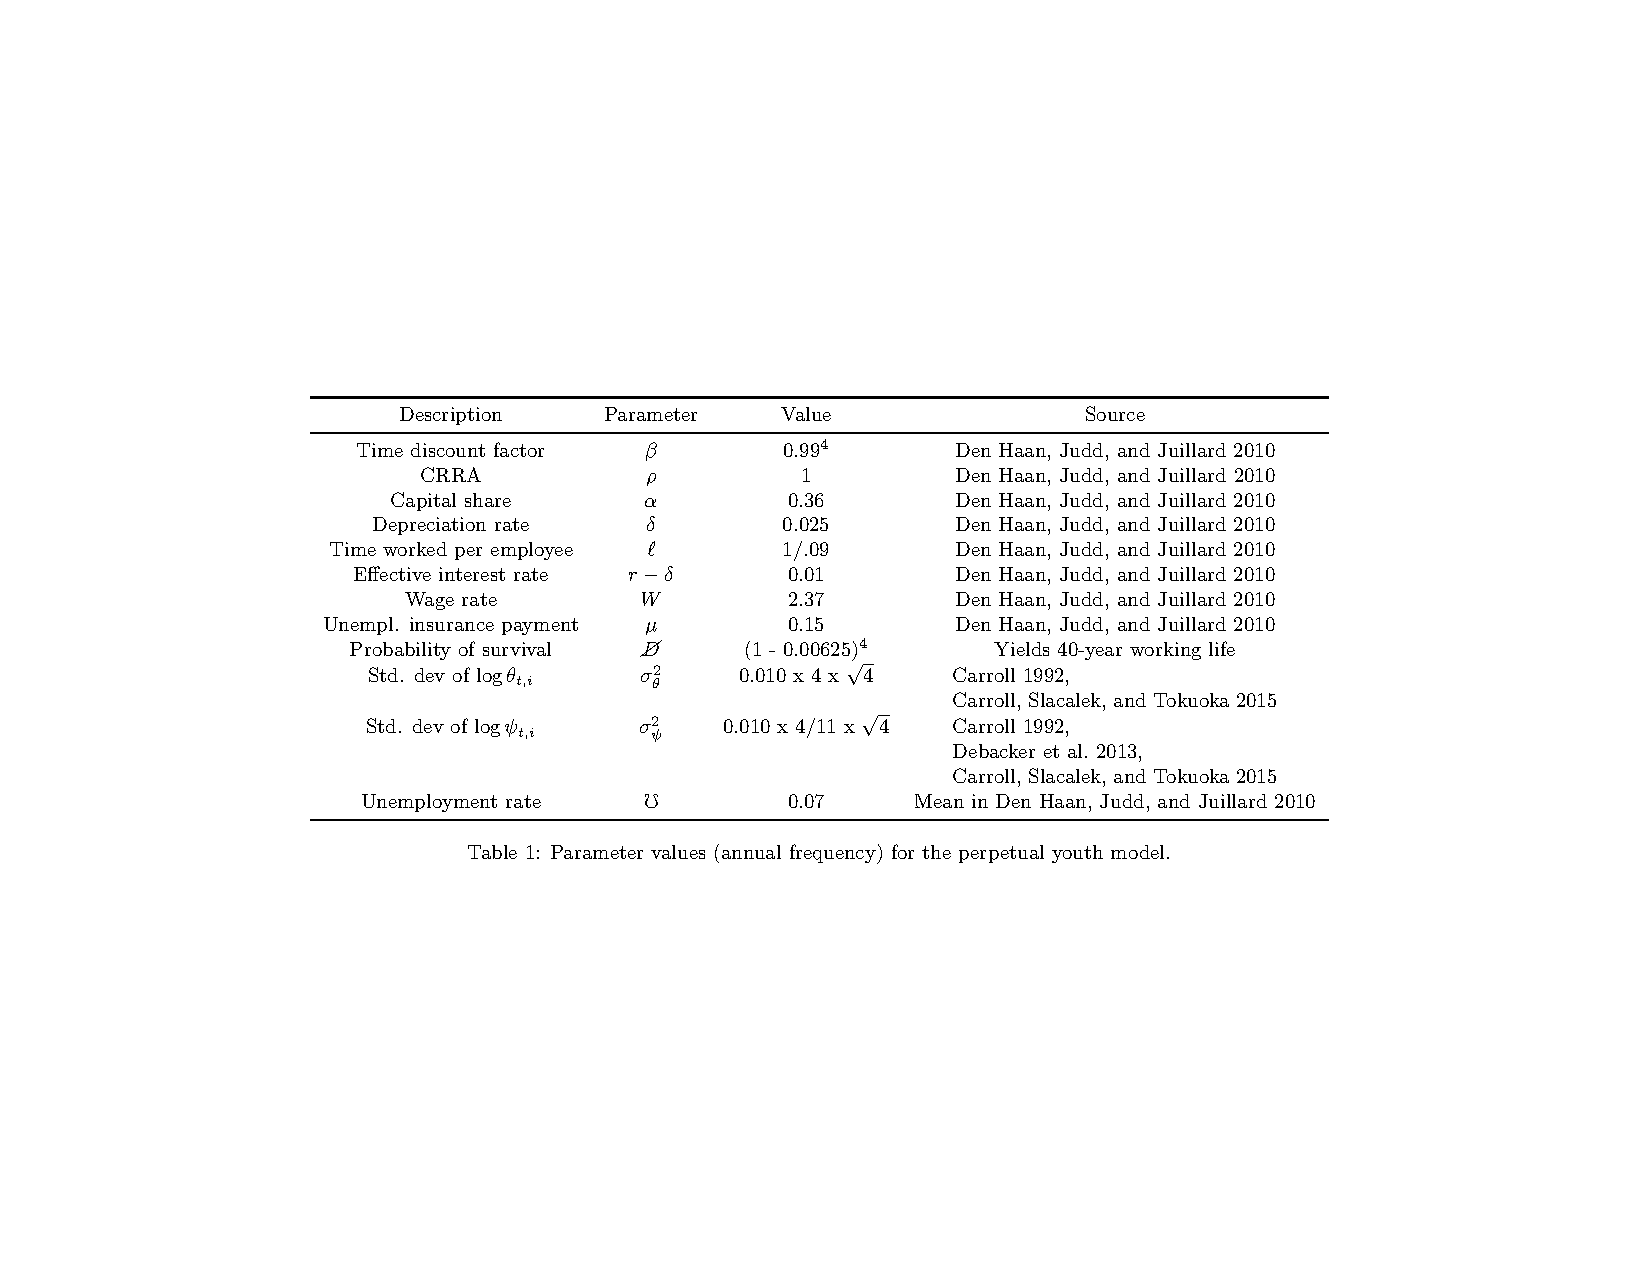
\includegraphics[width=.85\linewidth]{Tables/calibrationPY.pdf}
  \end{figure}
  \vfill

\end{frame}
%%%%%%%%%%%%%%%%%


\begin{frame}{Estimation procedure}

%\vspace{2.5mm}
%Goal: Find $R$ value(s) such that the simulated distribution of wealth best matches \textit{moments} of the household wealth data from the 2004 Survey of Consumer Finances (SCF).

Simulated method of moments (SMM) estimation for $R$ using 2004 SCF wealth data.

%\vspace{5mm}
  \begin{enumerate}
  \item No ex-ante heterogeneity: $R$\textit{-point} model
  \par Estimate a common rate of return across households by finding the $\grave{R}$ which matches the capital-to-output ratio $(\frac{K}{Y} = 7.47)$.
  \vspace{2.5mm}

  \item Ex-ante heterogeneity: $R$\textit{-dist} model
  \par Estimate  a \textbf{Uniform distribution} of returns across households by finding the $\grave{R}$,$\nabla$ which match empirical Lorenz targets, given $\frac{K}{Y}$.
  \end{enumerate}
  
  \centering
  \small
  \begin{tabular}{|c|c|}
\hline
Net worth percentile & Cumulative net worth \\
\hline
20th & -.18\%  \\
40th &  .95\% \\
60th &  5.3\% \\
80th &  17.09\% \\
\hline
\end{tabular}


\end{frame}
%%%%%%%%%%%%%%%%%

\section{Results}

\begin{frame}{How good is the fit?}

   \begin{columns}
    \column{0.5\textwidth}
    \centering
    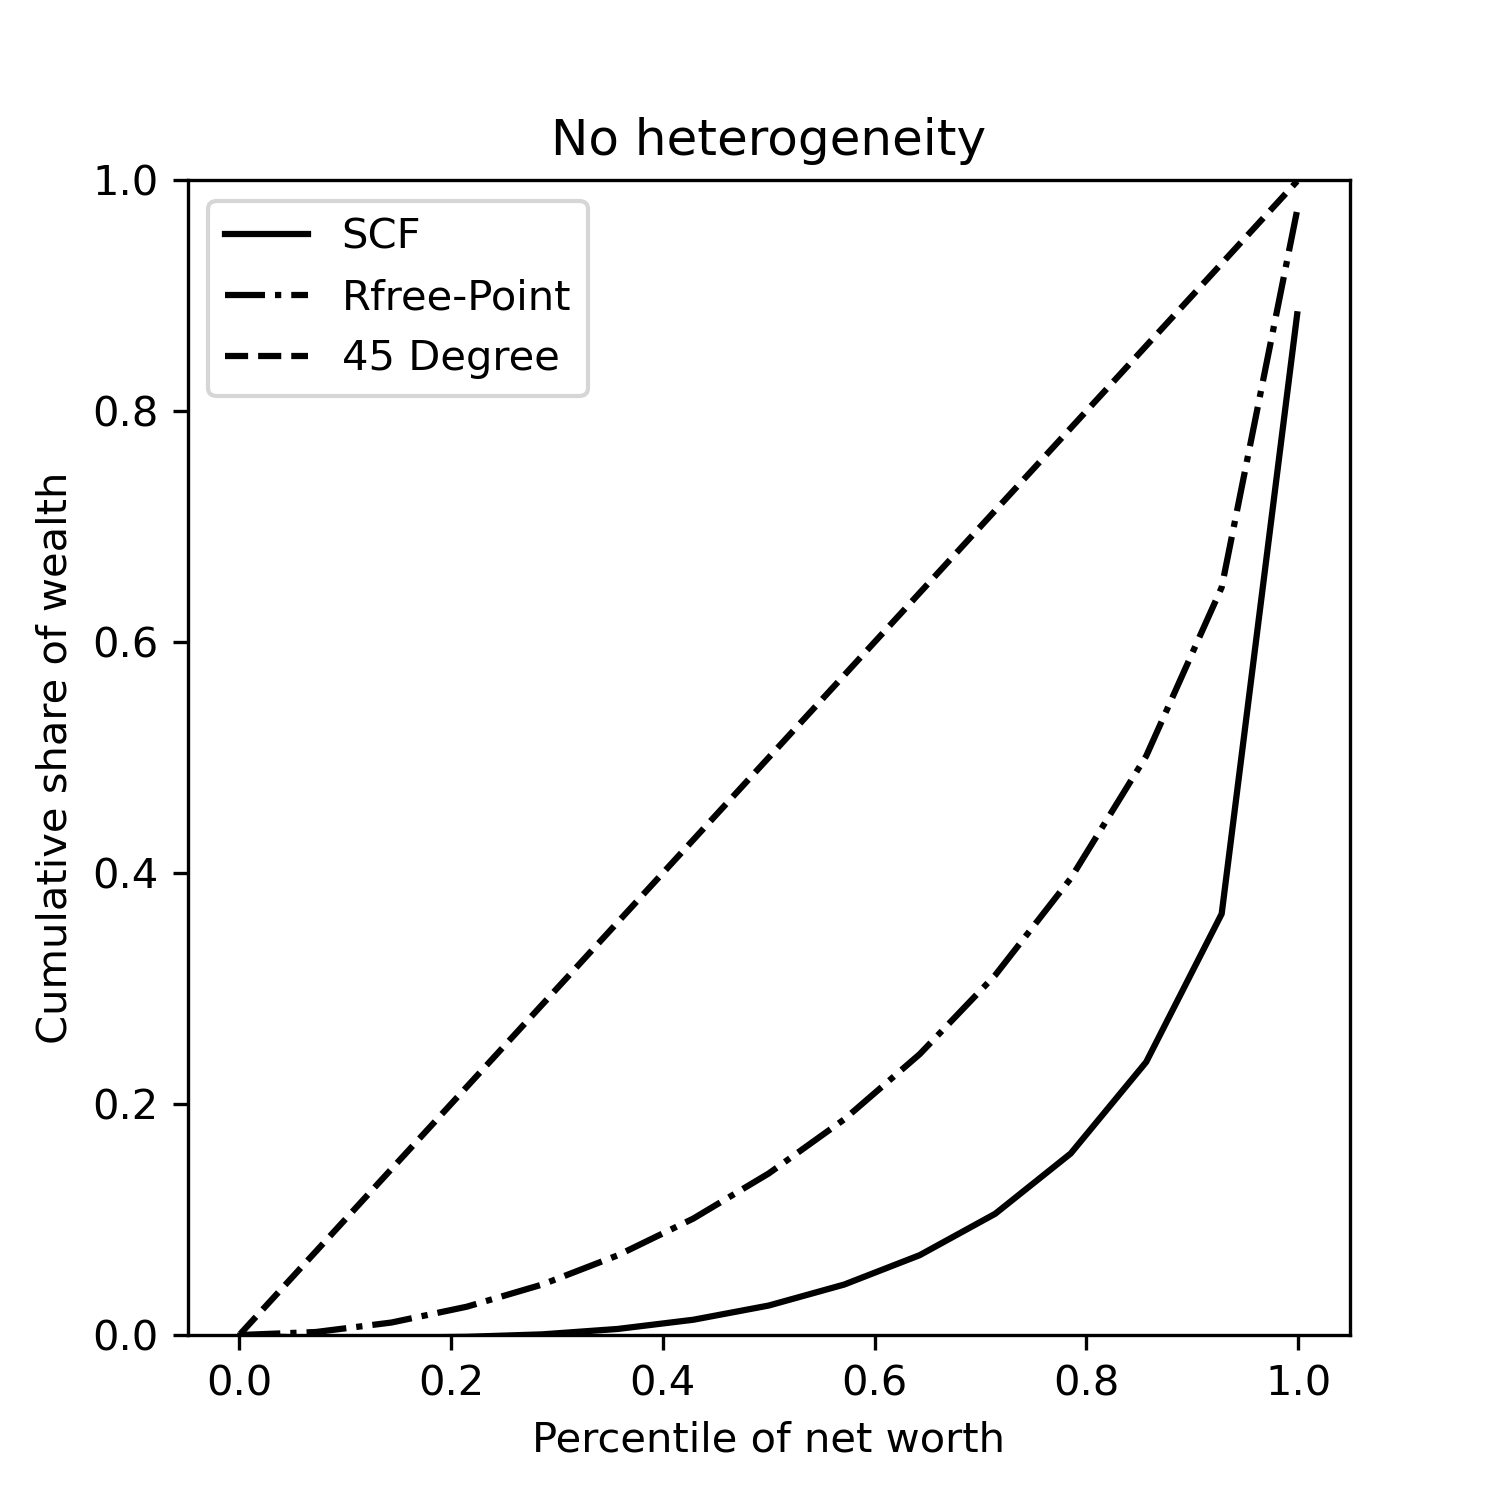
\includegraphics[width=\textwidth]{Figures/PYrrPointNetWorthPlot.png}

    \column{0.5\textwidth}
    \centering
    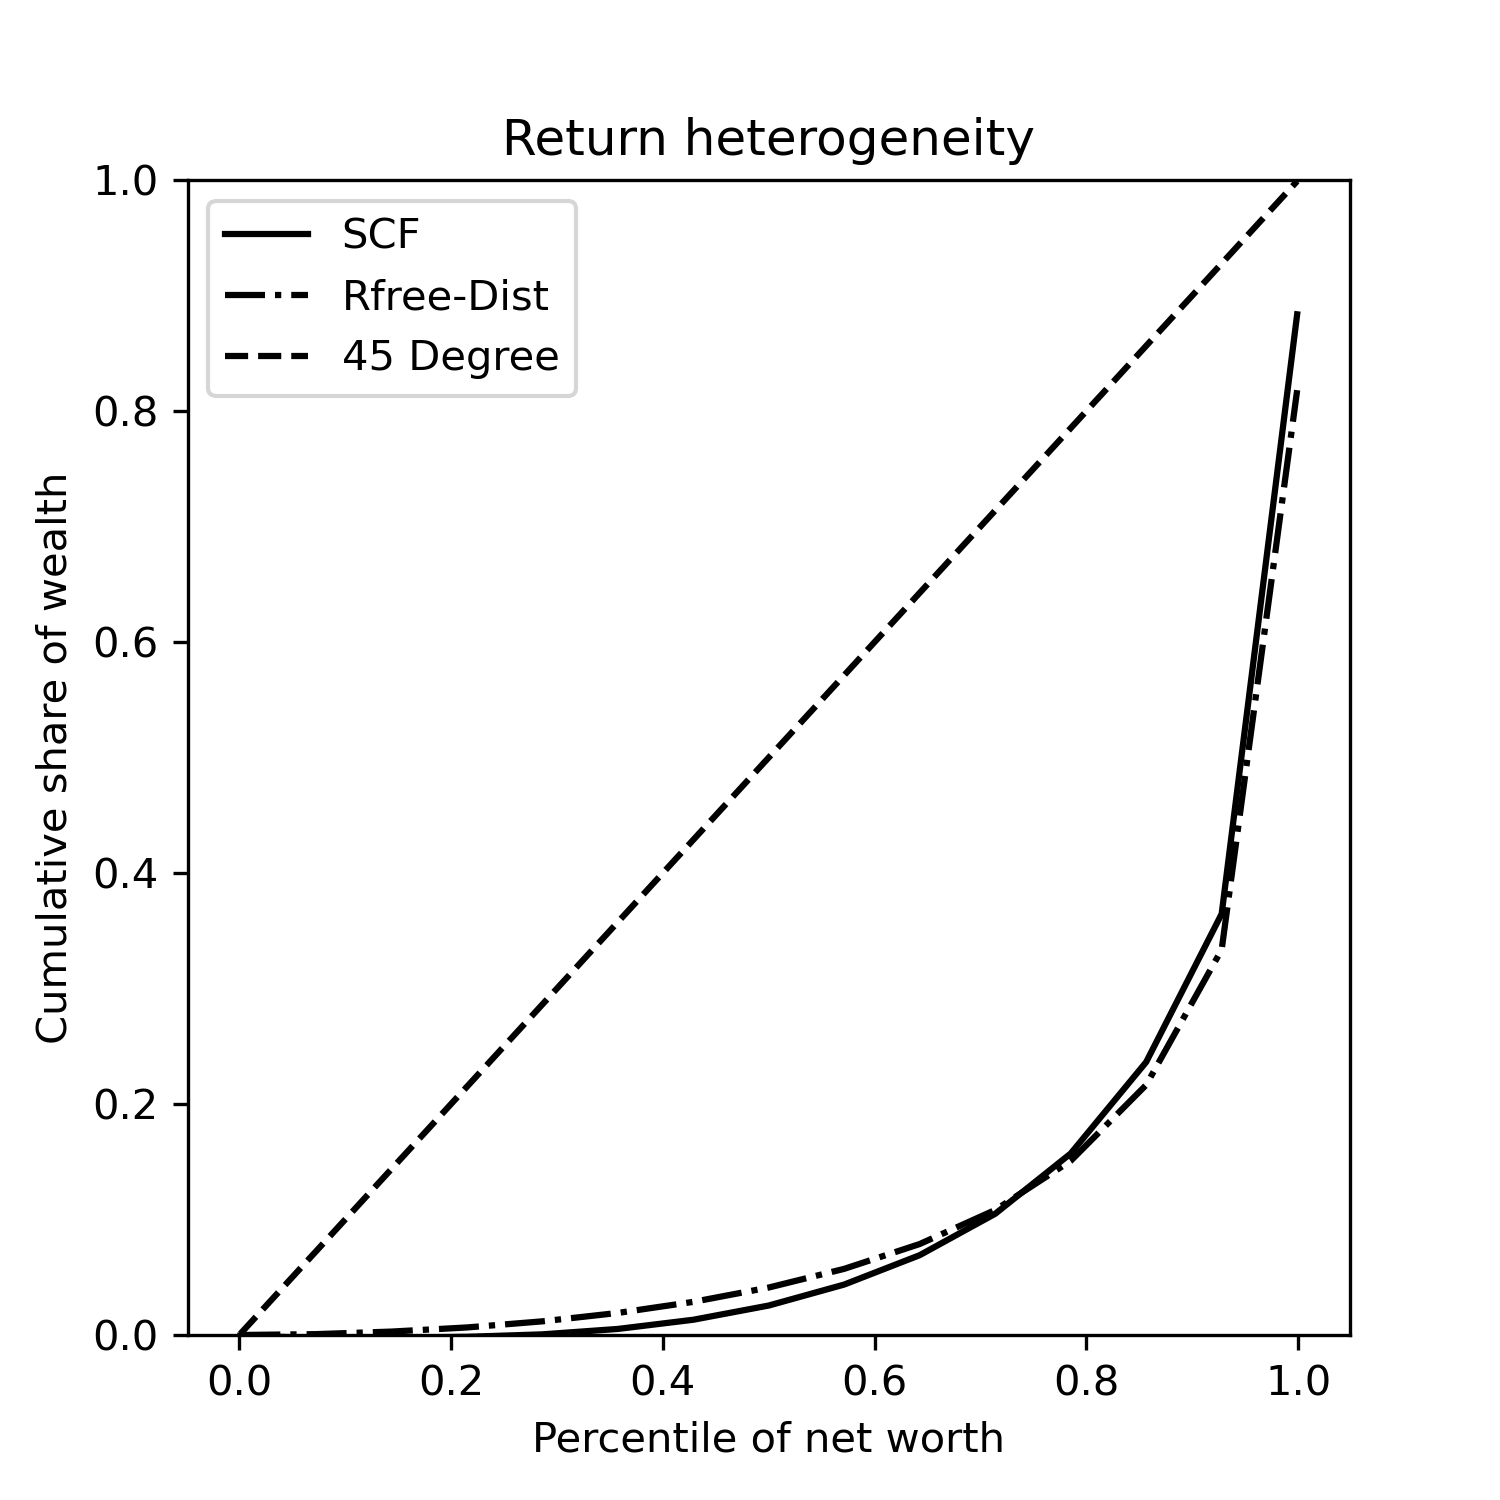
\includegraphics[width=\textwidth]{Figures/PYrrDistNetWorthPlot.png}

  \end{columns}

\end{frame}
%%%%%%%%%%%%%%%%

%%%%%%%%%%%%%%%

\begin{frame}{Lifecycle version of the model}
\begin{itemize}
\item Education cohort $e \in \{D, HS, C\}$
\item Initial wealth-to-income $k_0$ and income $p_0$ levels
\item Education-age dependent mortality rates
\par \parencite{Brown2007}
\item Modified labor income uncertainty $y_t = \xi_t \psi_t \overline{\psi}_{es} p_{t-1}$
\par \parencite{Cagetti2003}
\begin{itemize}
\item Education-age dependent shock variances
\par \parencite{Sabelhaus2010}
\end{itemize}
\end{itemize}
\end{frame}
%%%%%%%%%%%%%%%

\begin{frame}{Calibration}
  \vfill
   \begin{figure}
    \centering
    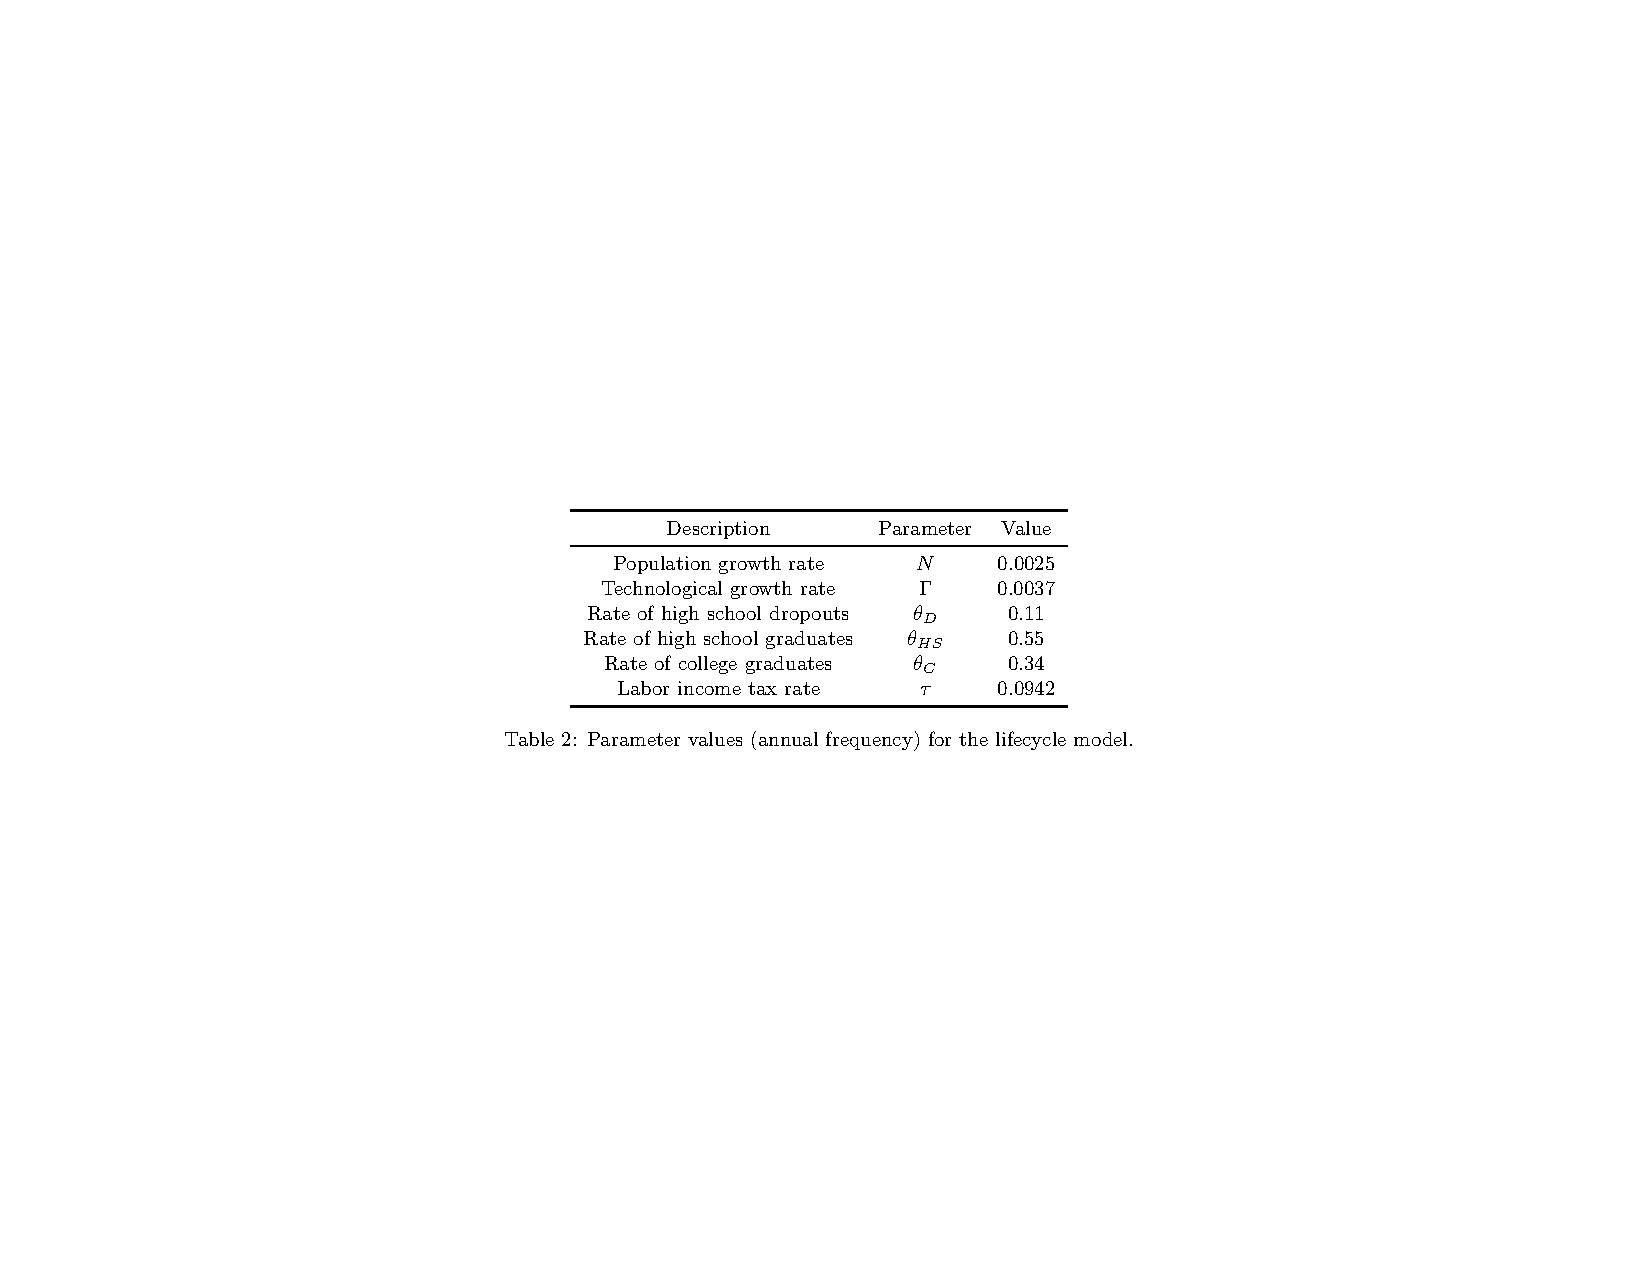
\includegraphics[width=.85\linewidth, scale=1.5]{Tables/calibrationLC.pdf}
  \end{figure}
  \vfill
\end{frame}

%%%%%%%%%%%%%%%%%%
\begin{frame}{How good is the fit?}
 \begin{columns}
    \column{0.5\textwidth}
    \centering
    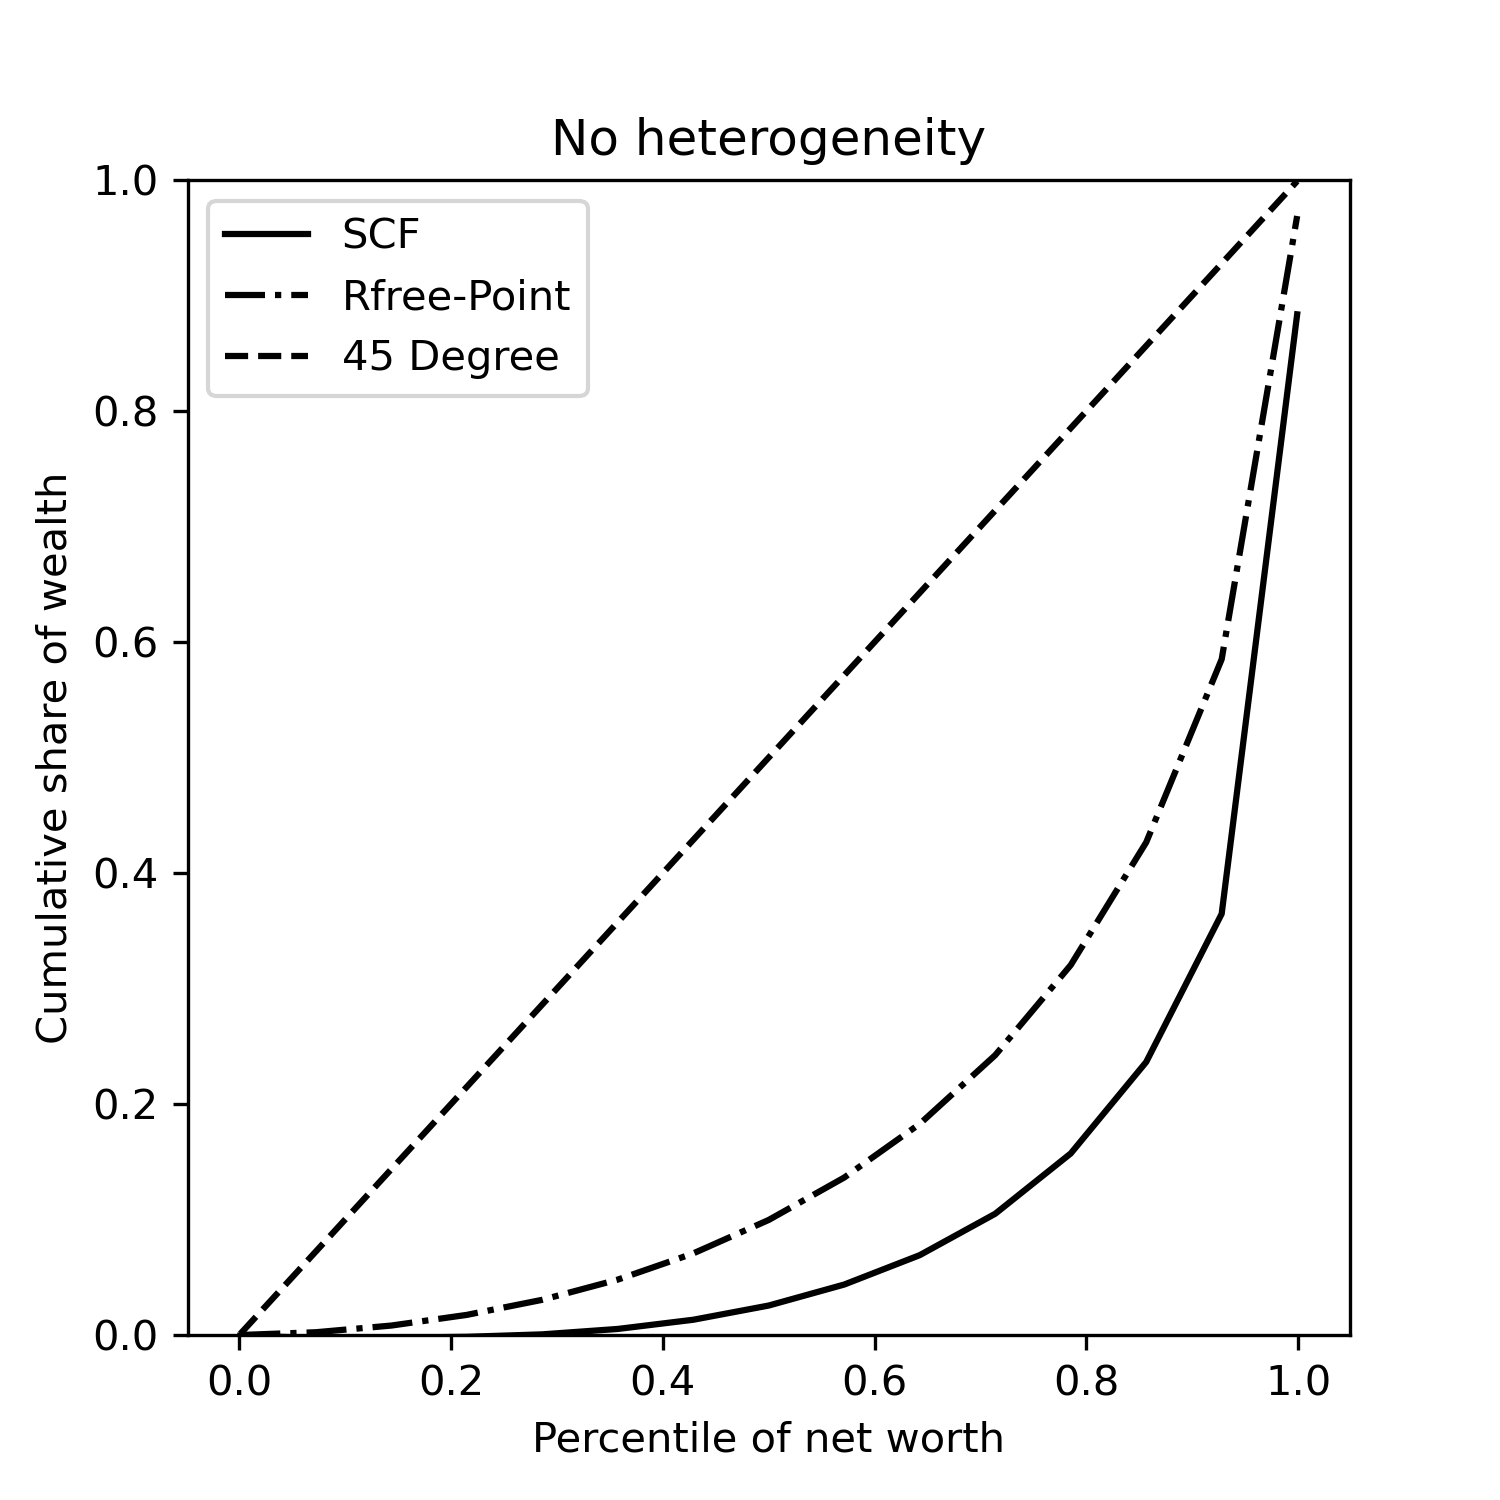
\includegraphics[width=\textwidth]{Figures/LCrrPointNetWorthPlot.png}

    \column{0.5\textwidth}
    \centering
    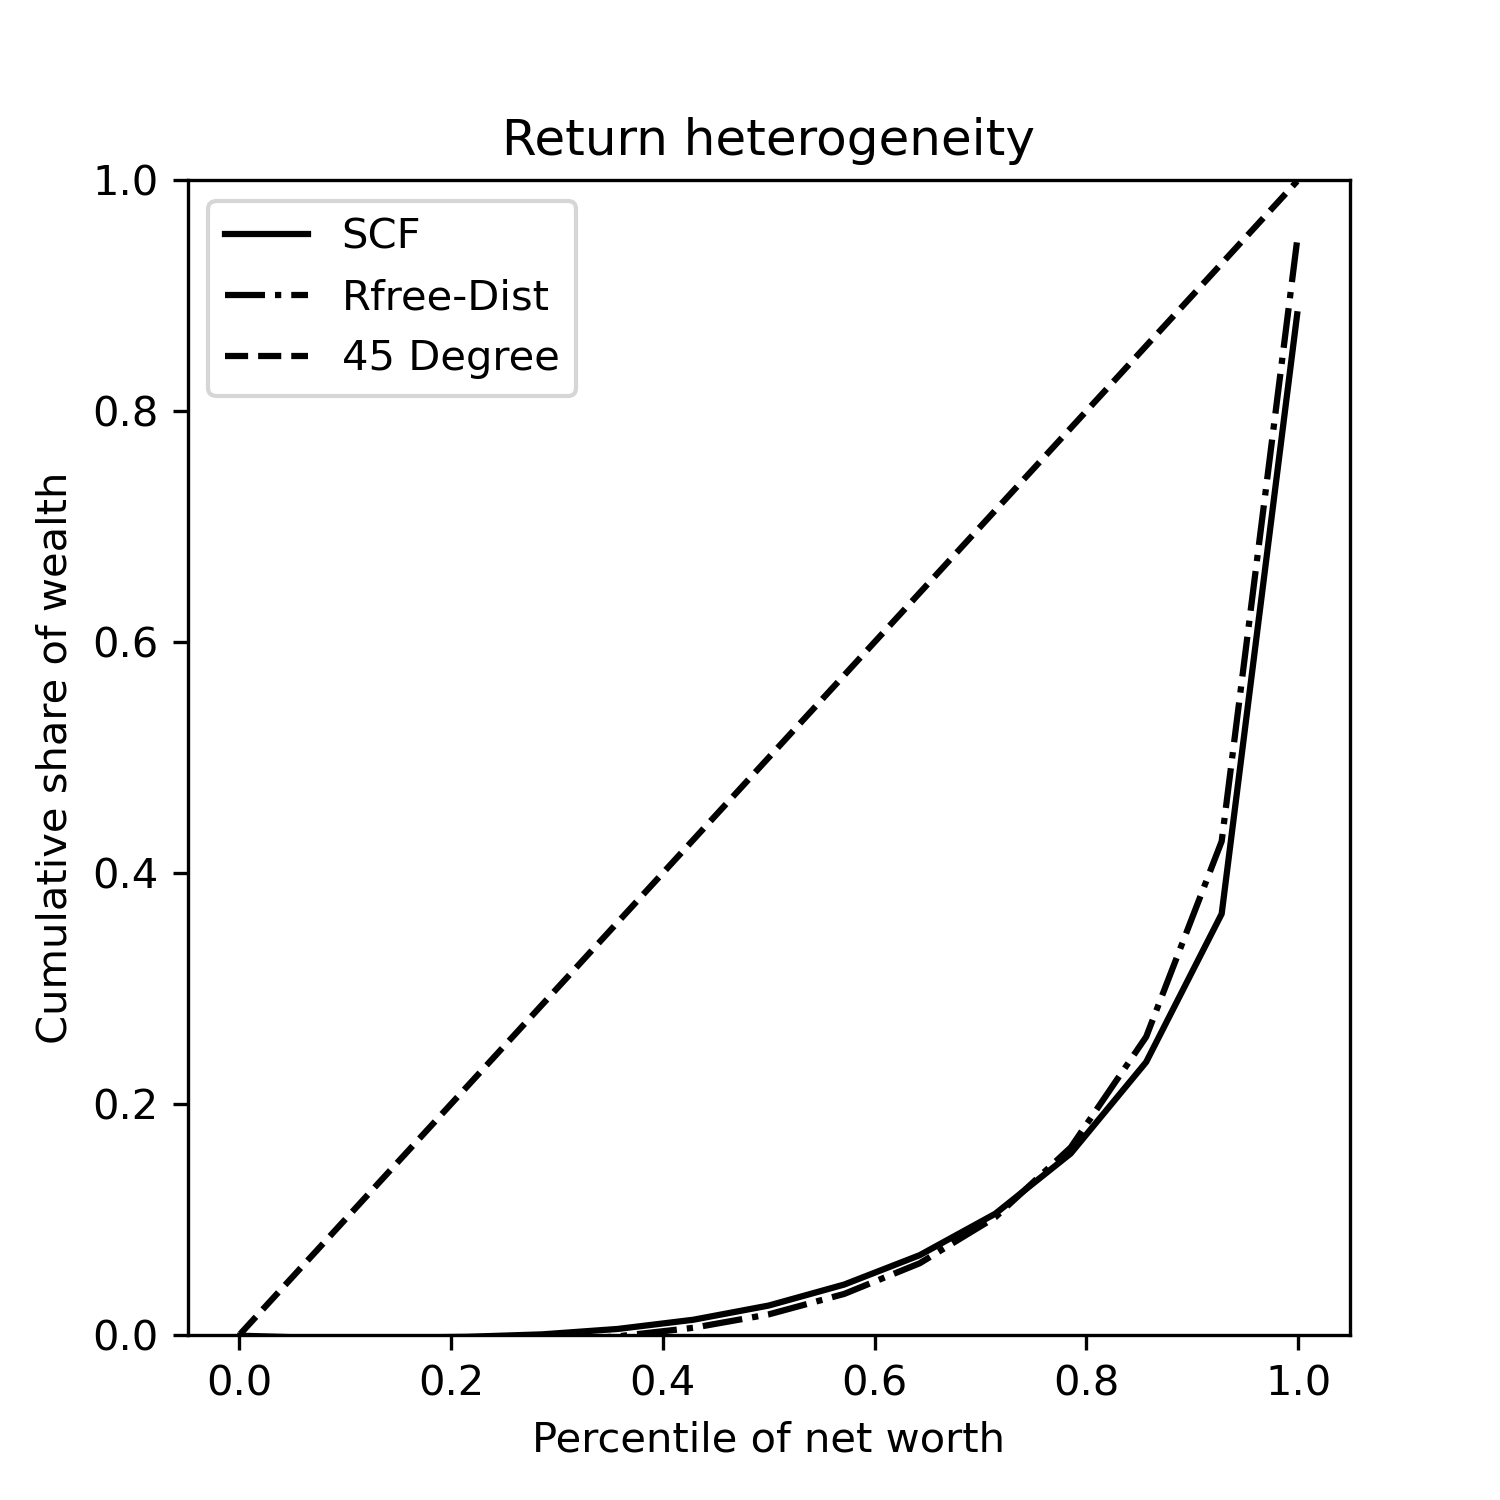
\includegraphics[width=\textwidth]{Figures/LCrrDistNetWorthPlot.png}

  \end{columns}
\end{frame}

%%%%%%%%%%%%%%%%

\begin{frame}{Model performance: returns distribution}
\centering

\begin{flushleft}
\par Empirical values from \cite{aflgdmlp20}
\end{flushleft}
    \begin{tabular}{|c|c|c|}
\hline
& Mean & St. Dev \\
\hline
Net worth (after tax) & 0.0365 & 0.0781  \\
\hline
\end{tabular}

\begin{flushleft}
\par Values from the structural estimation (uniform distribution for $R$)
\end{flushleft}
    \begin{tabular}{|c|c|c|}
\hline
& Mean & St. Dev \\
\hline
PY-Point & 0.071 & 0.0  \\
PY-Dist & 0.055  &  0.006  \\
LC-Point & 0.063 & 0.0  \\
LC-Dist & 0.049  &  0.010  \\
\hline
\end{tabular}

\end{frame}
%%%%%%%%%%%%%%%%%%

\begin{frame}{Model performance: untargeted moments}
\centering
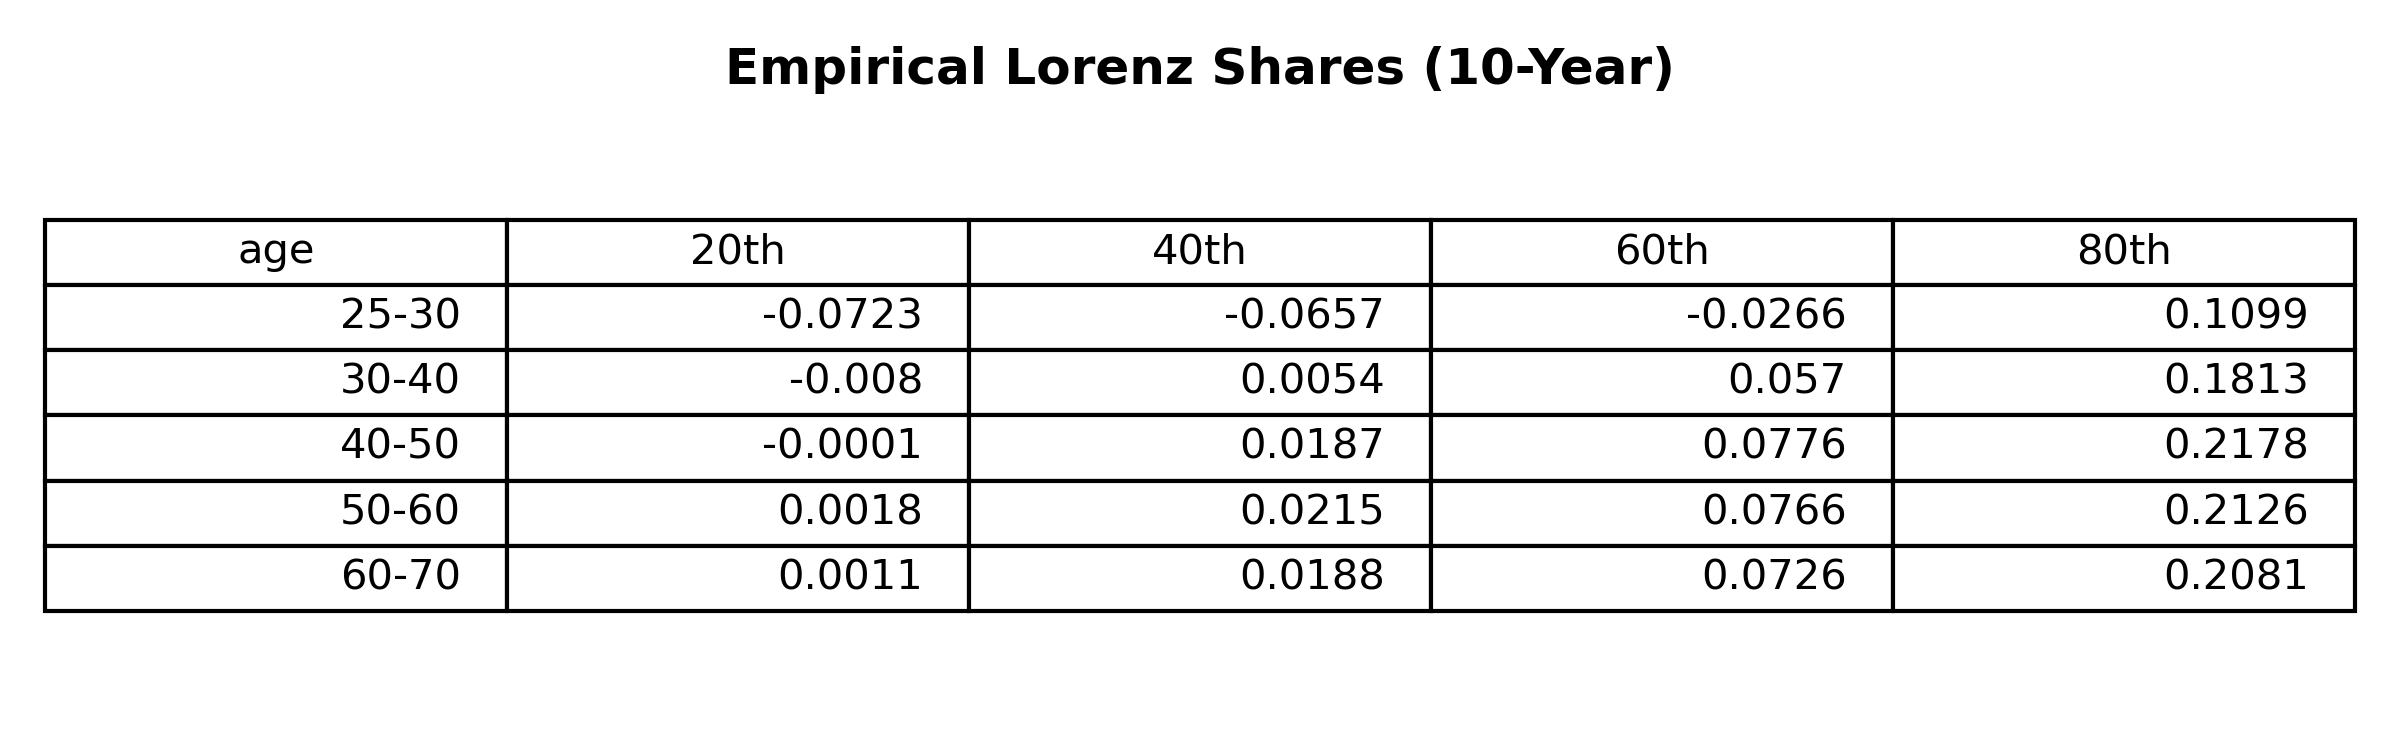
\includegraphics[width=0.8\textwidth]{Tables/Emp_Lorenz_10yr_LCrrDistNetWorth.png}

%\vspace{0.5cm} % vertical space between the two tables/images

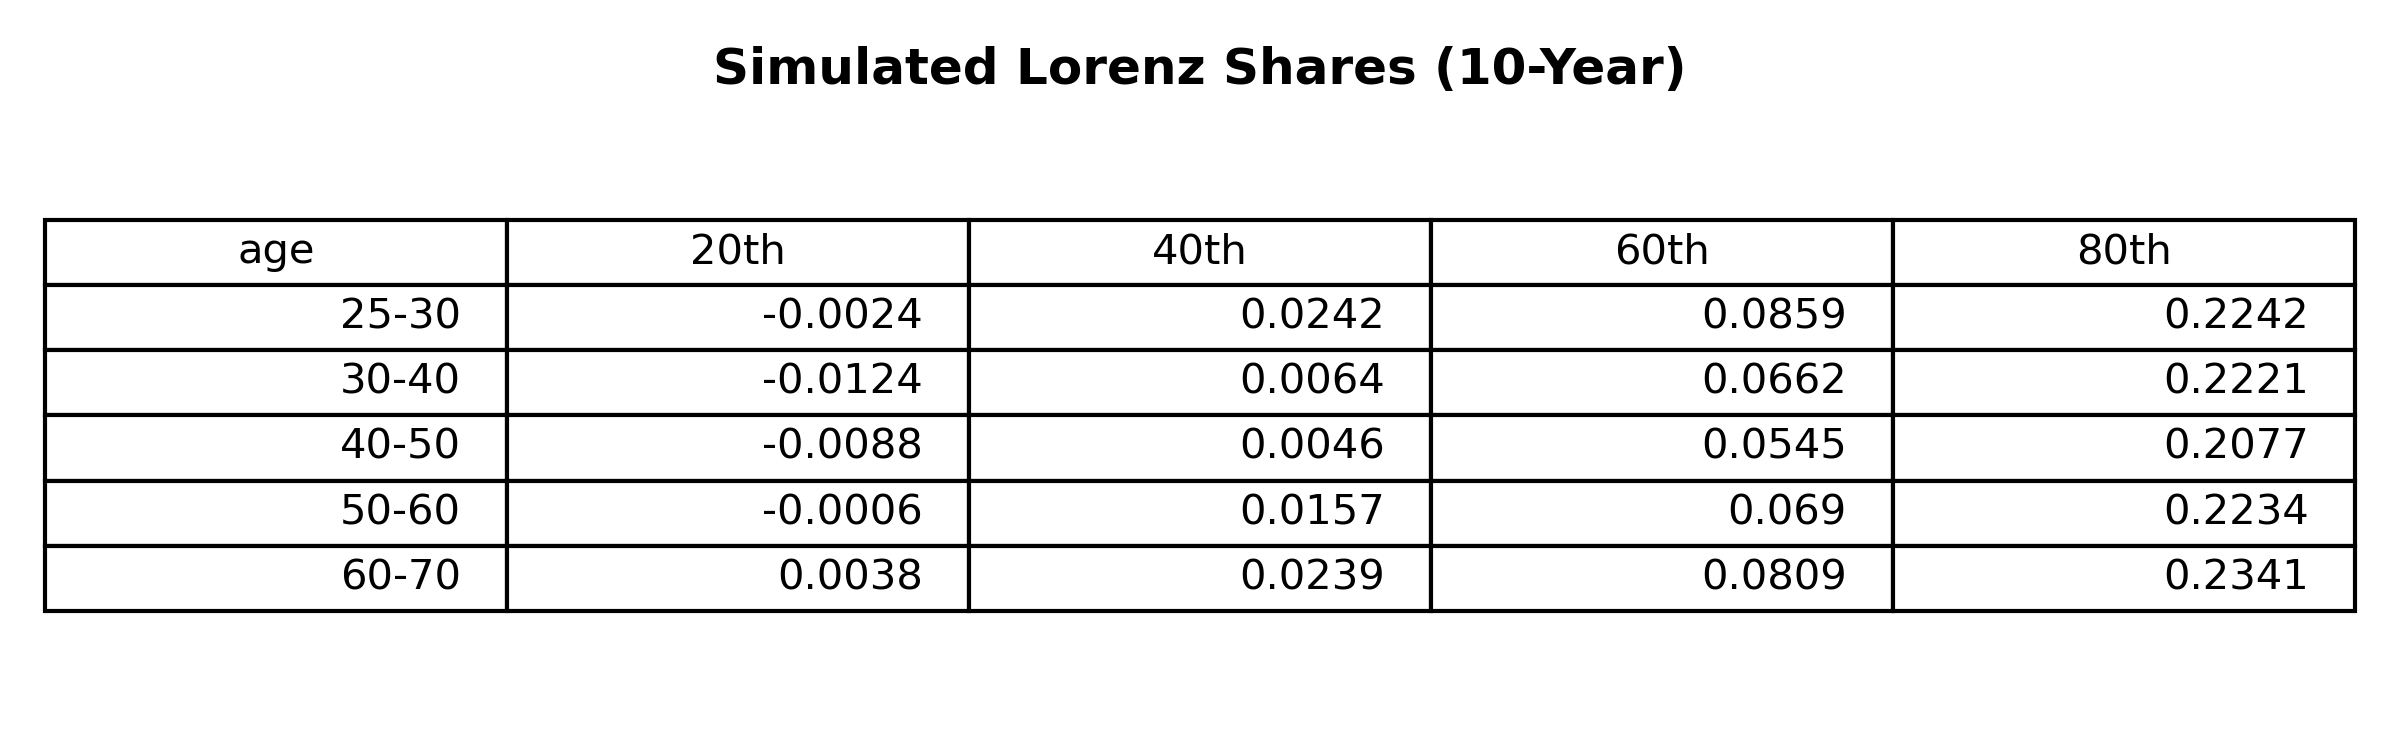
\includegraphics[width=0.8\textwidth]{Tables/Sim_Lorenz_10yr_LCrrDistNetWorth.png}

\end{frame}
%%%%%%%%%%%%%%%%%%


\subsection{Concluding Remarks}

\begin{frame}{Work to be done}

       \begin{enumerate}
       \item Robustness checks
       \begin{itemize}
      \item Plausible parameter values for time preferences and risk aversion
      \item Different measures of wealth (liquid and/or financial)
      \end{itemize}
      \end{enumerate}

\end{frame}
%%%%%%%%%%%%%%

%\subsection{Concluding Remarks}
%
%\begin{frame}{Work to be done}

 %      \begin{enumerate}
 %      \item Robustness checks
  %     \begin{itemize}
%      \item Plausible parameter values for time preferences and risk aversion
%      \item Different measures of wealth (liquid and/or financial)
%      \end{itemize}
 %     \end{enumerate}

 %   \end{frame}
%%%%%%%%%%%%%


\begin{frame}[allowframebreaks]{References}
  \printbibliography
\end{frame}

\end{document}




